\section{Text-Based Retrieval-Augmented Generation}
\label{sec:text_rag}

Document-level question answering faces two core challenges: LLMs are limited by context length for long or multi-document inputs, and pure generative models are prone to hallucinations without external evidence constraints. Retrieval-Augmented Generation (RAG) addresses these challenges by combining information retrieval with text generation. This section traces the five-stage evolution of RAG paradigms (\cref{fig:rag_evolution}): retrieve-then-generate, structure and reasoning-guided RAG, graph-enhanced RAG, multimodal RAG, and agentic RAG.

\subsection{Retrieval-Augmented Generation}

Early RAG followed the classic ``retrieve-then-generate'' paradigm, improving DocQA performance through evidence recall quality and multi-hop support.

Triple-Fact Retriever \cite{wu2022triple} improved cross-document evidence path accuracy by extracting structured triple facts and aggregating evidence hop by hop. Multi-Document Question Answering with Lightweight Embeddings \cite{aitymbetov2024multi} employed two-stage retrieval combining BM25 coarse-ranking with embedding-based re-ranking. Zero-Shot Complex Question-Answering on Long Scientific Documents \cite{wang2025zero} integrated RAG with question decomposition and multi-hop reasoning without task-specific fine-tuning. DR-RAG \cite{hei2024dr} mitigated evidence omission through dynamic document relevance modeling.

\subsection{Structure and Reasoning-Guided RAG}

Subsequent research focused on utilizing LLM reasoning capabilities and document structural information to build structure-aware retrieval frameworks.

DocReLM \cite{wei2024docrelm} fine-tuned retrievers by generating domain-specific training data and citation networks. Advanced Chain-of-Thought Reasoning for Parameter Extraction \cite{chen2025advanced} introduced improved CoT reasoning through targeted document retrieval and iterative optimization. Semi-Structured Chain-of-Thought \cite{su2024semi} unified parametric knowledge, structured knowledge graphs, and unstructured text retrieval.

For long documents, Beyond Chunking \cite{chen2025chunkingdiscourseawarehierarchicalretrieval} utilized Rhetorical Structure Theory for discourse-level modeling and hierarchical retrieval. PdfTriage \cite{saad2024pdftriage} explicitly modeled structural meta-information (pages, sections, tables) for structured long-document QA. Knowledge Graph Prompting for Multi-Document QA \cite{wang2024knowledge} enhanced global consistency through cross-document knowledge graphs.

\subsection{Graph-Enhanced RAG}

Recent research has treated retrieval as a decision-making step directly driven by the reasoning process, utilizing graph structures for evidence organization.

GraphRAG \cite{edge2024graphrag} proposed a graph-enhanced retrieval framework using knowledge graphs and community detection for global, cross-document queries. LightRAG \cite{guo2024lightrag} addressed computational overhead through a lightweight dual-level index architecture. HyperGraphRAG \cite{he2024hypergraphrag} introduced hypergraph structures to model n-ary relations, preserving semantic integrity of complex events.

Dynamic retrieval mechanisms improved evidence continuity. Spreading Activation for Document Retrieval \cite{pavlovic2025leveraging} enabled activation propagation along evidence chains. GARLIC \cite{wang2024garlic} constructed hierarchical weighted graphs for dynamic retrieval path control. HiQA \cite{chen2024hiqa} transformed documents into hierarchical structures with cascading metadata. BookRAG \cite{wang2025bookrag} built BookIndex fusing logical hierarchy trees and entity-relationship graphs.

Multi-hop reasoning was enhanced through iterative expansion. Chain of Retrieval \cite{park2025chain} drove iterative expansion via multi-aspect decomposition and post-order aggregation. Enhancing Document-Level QA via Multi-Hop RAG with LLaMA 3 \cite{huang2025enhancing} integrated dense retrieval, context fusion, and multi-hop mechanisms.

\begin{figure*}[t]
\centering
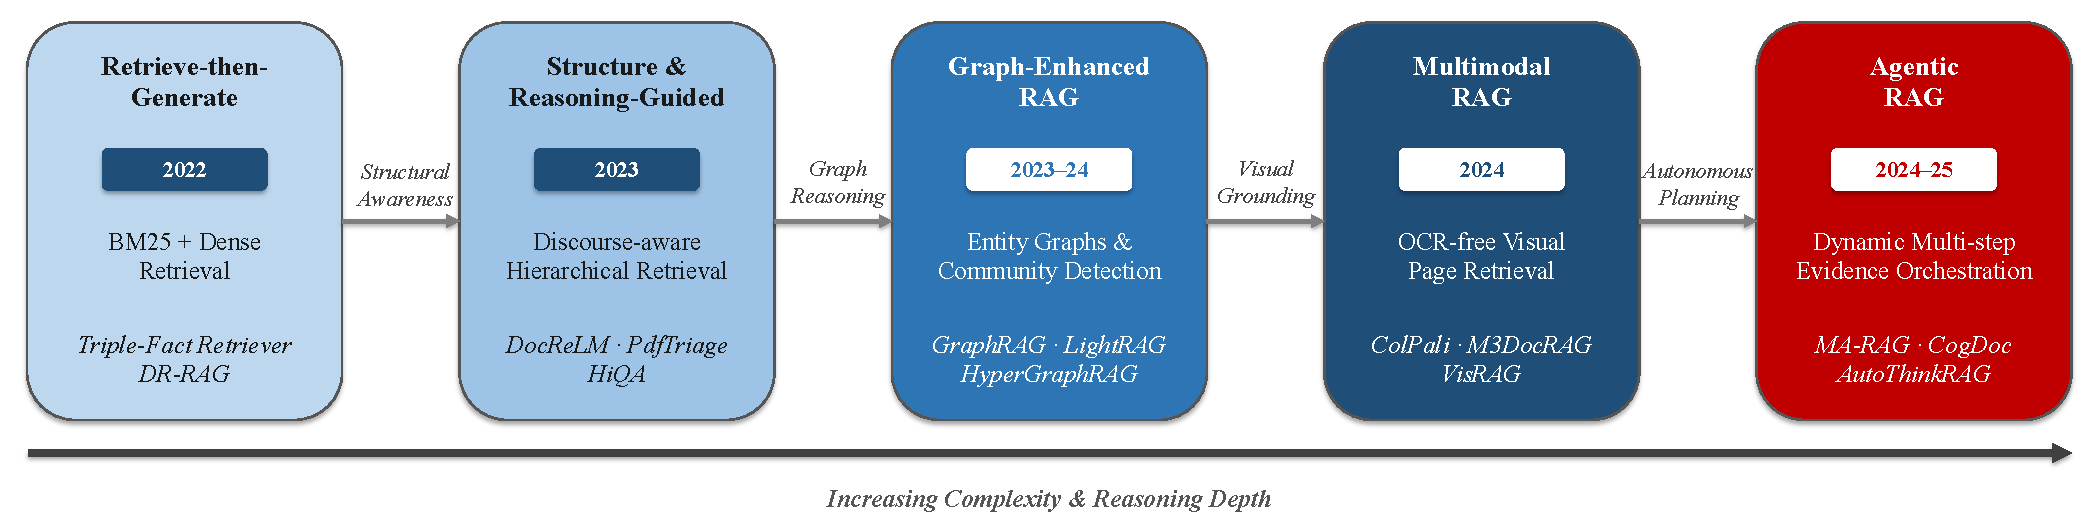
\includegraphics[
    width=0.95\textwidth,
    height=0.38\textheight,
    keepaspectratio,
    trim=0cm 0cm 0cm 0cm,
    clip
]{figs/fig06.pdf}
\caption{Five-stage evolution of retrieval-augmented generation paradigms for document question answering, progressing from Retrieve-then-Generate (2022) through Structure and Reasoning-Guided RAG (2023), Graph-Enhanced RAG (2023--2024), Multimodal RAG (2024), and Agentic RAG (2024--2025), with representative systems listed at each stage and increasing complexity and reasoning depth indicated along the horizontal axis.}
\label{fig:rag_evolution}
\end{figure*}

\subsection{End-to-End Document Question Answering}

Beyond retrieval-augmented approaches, end-to-end document QA has evolved through attention mechanisms, graph-based reasoning, and LLM-era methods.

\subsubsection{Early Attention Mechanisms}

Dynamic Coattention Networks \cite{dynamiccoattention2017} proposed co-attention strategies capturing bidirectional interaction between questions and documents. Coarse-to-fine question answering \cite{coarsetofine2017} pioneered a two-stage framework: first retrieving relevant sentences, then extracting precise answers. EA Reader \cite{eareader2019} utilized multi-space context fusion for improved cloze-style QA.

\subsubsection{Graph Structures and Global Information}

Graph Neural Networks became the core paradigm for connecting discrete evidence. Question Answering by Reasoning Across Documents with GCNs \cite{gcnmultihop2019} utilized entity-based Graph Convolutional Networks for multi-hop tasks. Identifying Supporting Facts with Document Graph Networks \cite{dgn2019} shifted focus to explicit identification of supporting facts through sentence-level document graphs.

Explainable frameworks improved interpretability. Exploiting Explicit Paths \cite{explicitpaths2019} scored and selected evidence paths. Multi-hop Question Answering via Reasoning Chains \cite{reasoningchains2020} used reasoning chains as intermediate explicit variables. Select, Answer and Explain \cite{sae2020} simultaneously generated answers and evidence rationales.

\subsubsection{Task Generalization and the LLM Era}

Multi-hop reasoning expanded to broader tasks. Multi-Hop Transformer \cite{multihoptransformer2021} introduced multi-hop reasoning to translation. Syntax-enhanced multi-hop reasoning \cite{syntaxmultihop2024} advanced document-level relation extraction. MemSum-DQA \cite{memsumdqa2023} streamlined QA model inputs through extractive summarization while preserving evidence integrity.

Recent work explores LLM capabilities for document understanding. Effect of Document Packing \cite{documentpacking2025} examines how document organization affects multi-hop reasoning performance in LLMs.
